% TrueLift: the end-to-end report, IEEE conference format.
% Build: python submission/src/build.py report   (fills every number from reports/; see build.py)
\documentclass[conference]{IEEEtran}
\usepackage{fontspec}
\setmainfont{texgyretermes}[Extension=.otf,UprightFont=*-regular,BoldFont=*-bold,ItalicFont=*-italic,BoldItalicFont=*-bolditalic]
\usepackage{unicode-math}
\setmathfont{texgyretermes-math.otf}
\usepackage{newunicodechar}
\usepackage{tfrupee}
\newunicodechar{₹}{\rupee{}}
\usepackage{graphicx}
\usepackage{booktabs}
\usepackage{array}
\usepackage{xcolor}
\usepackage{tikz}
\usetikzlibrary{positioning,arrows.meta,calc}
\usepackage{pgfplots}
\pgfplotsset{compat=1.18}
\usepackage[hidelinks]{hyperref}
\usepackage{cite}
\definecolor{tlblue}{HTML}{2A78D6}
\definecolor{tlgrey}{HTML}{B9B6B0}
\definecolor{tldark}{HTML}{6F6B66}
\input{numbers.tex}
\newcolumntype{L}[1]{>{\raggedright\arraybackslash}p{#1}}
\newcolumntype{R}[1]{>{\raggedleft\arraybackslash}p{#1}}

\begin{document}

\title{TrueLift: Forecasting, Targeting and Measuring\\Restaurant-Funded Discounts by the Orders They Create}

\author{\IEEEauthorblockN{Yash Goyal, Bhavay Goyal, Kshitish Madbhavi}
\IEEEauthorblockA{Team Banana, Indian Institute of Technology Gandhinagar, Gujarat, India\\
IITGN $\times$ Eternal Hackathon, Round 2, November 2026\\
Live demo: \url{https://yashg1836.github.io/truelift/} \quad Code: \url{https://github.com/YashG1836/truelift}}}

\maketitle

\begin{abstract}
Food-delivery platforms judge a restaurant's discount by the orders that use it, not by the orders it
creates. Since August 2026 every restaurant-funded offer on Zomato starts only after the owner approves
it with a one-time password (OTP), so an owner who cannot see whether an offer pays has every reason to
stop approving it. We present TrueLift, which adds four calls to the offer flow Zomato already has: a
forecast of the extra orders and profit an offer will create, with a range, shown before approval; a
serving rule that shows the discount only to customers it is likely to move and holds out a random
tenth of the eligible ones; an itemised payout; and a weekly measurement that combines the
restaurant's own control group with a model learned from all restaurants. The uplift model is a
T-learner on gradient-boosted trees. In a simulated market of 300 real Bengaluru listings, where the
true effect of every offer is known, \V{tl_pay} of \V{tl_offers} TrueLift offers pay for themselves
against \V{bl_pay} of 300 blanket offers. Restaurants' profit rises by \V{readme_tl_market} a week over
no offers, against \V{readme_bl_market} with blanket offers, while they give \V{readme_less_discount}
less discount, and Zomato's commission is higher too. After four weeks the weekly 80\% range contains the true effect for
\V{devlog_cov_4} of offers. On two public randomised datasets the method wins on some outcomes and not
on others, and we report both. A working prototype with a guided demo is public.
\end{abstract}

\begin{IEEEkeywords}
uplift modelling, causal inference, randomised holdout, food delivery, promotion measurement,
two-sided marketplaces
\end{IEEEkeywords}

\section{Introduction}

Discounts are one of the largest costs on a food-delivery platform. Eternal, Zomato's parent, spent
₹1,138 Cr on advertising and sales promotion in the quarter to September 2026, 41\% more than a year
earlier, while its food-delivery business earned an adjusted EBITDA of 5.5\% of order value
\cite{eternal}. Restaurants fund many of these discounts themselves. In July and August 2026 restaurant
associations in Bengaluru objected to deductions made without clear consent; Zomato agreed that
restaurant-funded campaigns become opt-in and start only after the owner approves them by OTP
\cite{angelone,theweek}.

Consent turns a measurement gap into a business problem. An offer report today counts the orders that
used an offer and the sales they brought. Whether the offer paid depends on a number no report shows:
the share of those orders that would not have happened without it. A regular who orders every week
and now gets ₹60 off is not an extra order; the restaurant simply earns less on it. An owner who cannot
see that share approves blind, and under the OTP rule an owner who has lost money on blind approvals can
decline the next one.

TrueLift closes the gap inside the flow that already exists. This report makes four contributions:
\begin{enumerate}
\item an exact statement, in rupees, of when a restaurant-funded discount pays (Section~\ref{sec:money});
\item four calls that fit Zomato's partner and customer apps without new screens (Section~\ref{sec:design});
\item a forecasting, targeting and weekly measurement method that works for restaurants with about
fifty orders a week, with a pause rule that stays valid however often the owner looks (Section~\ref{sec:method});
\item an evaluation in a simulated market with known truth, against strong baselines, under eight varied
assumptions and on real randomised data, with a public prototype (Sections~\ref{sec:setup}--\ref{sec:prototype}).
\end{enumerate}

\section{Related Work}

\emph{Uplift modelling} estimates the change in a person's response caused by a treatment, so that
the treatment goes to those it changes. Meta-learners build such estimates from standard classifiers:
the S-learner adds the treatment as an input, the T-learner fits one model per group, and the X-learner
combines them \cite{kunzel}. Rankings are scored with the Qini curve \cite{radcliffe}. Public randomised
benchmarks include Criteo's advertising holdouts \cite{criteo} and Hillstrom's e-mail test \cite{hillstrom}.

\emph{Online experiments} supply the measurement side. Regression adjustment with pre-experiment data
(CUPED) reduces the variance of a treatment effect estimate \cite{cuped}. Confidence sequences give
intervals that remain valid at every look, so a running test can be checked weekly without inflating
false alarms \cite{howard}. Ghost ads measure advertising effects with a control group that is never
shown the ad \cite{ghostads}; DoorDash uses ghost ads to measure what its restaurant ads add \cite{doordash}.

\emph{Industry practice} already targets discounts. Swiggy's Discount Self Serve lets about one lakh
restaurants pick customer segments and track performance \cite{swiggy}; Zomato's Brand Packs reward
repeat orders \cite{brandpacks}. These tools decide who \emph{can} see an offer and report how often it
was used. None of them forecasts or measures what a restaurant-funded offer \emph{caused}, at the point
where the owner consents.

\section{When a Discount Pays}
\label{sec:money}

Table~\ref{tab:order} gives the money of one ₹400 order under Zomato's usual terms as we model them:
commission of 25\% of the bill, 18\% GST on the commission, and food and packaging at 37\% of the menu
price. The same code computes every rupee in the service and the demo.

\begin{table}[t]
\caption{The money of one ₹400 order}
\label{tab:order}
\centering\footnotesize
\begin{tabular}{@{}lrr@{}}
\toprule
& Full price & ₹60 off, paid by the restaurant \\
\midrule
Food sales & \V{ord_full_basket} & \V{ord_disc_basket} \\
Discount & -- & $-$\V{ord_disc_discount} \\
Commission (25\% of the bill) & $-$\V{ord_full_commission} & $-$\V{ord_disc_commission} \\
GST on commission (18\%) & $-$\V{ord_full_gst_on_commission} & $-$\V{ord_disc_gst_on_commission} \\
Food and packaging (37\%) & $-$\V{ord_full_food_cost} & $-$\V{ord_disc_food_cost} \\
\midrule
\textbf{Restaurant keeps} & \textbf{\V{ord_full_restaurant_profit}} & \textbf{\V{ord_disc_restaurant_profit}} \\
Zomato's gross commission & \V{ord_full_zomato_gross} & \V{ord_disc_zomato_gross} \\
\bottomrule
\end{tabular}
\end{table}

Let $f$ be the share of the orders using an offer that would not have happened without it. The
restaurant gains its discounted profit $\pi_d$ on those and loses $\pi_f-\pi_d$ on all the others, where
$\pi_f$ is its full-price profit. It breaks even when
\begin{equation}
f^{*} = 1-\frac{\pi_d}{\pi_f} = 1-\frac{\text{\V{keeps_discounted}}}{\text{\V{keeps_full}}} = \text{\V{break_even_15}}.
\end{equation}
Table~\ref{tab:breakeven} repeats this for other discount sizes. If commission is charged on the bill
\emph{before} the discount (third-party calculators disagree), ₹60 off leaves \V{pre_discount_keeps}
and the break-even rises to \V{pre_discount_break_even}. Percentage offers with a cap concentrate the
headline percentage on small orders, where the restaurant keeps least: ``40\% off up to ₹80'' pays only
if \V{pct_small_order} of the ₹150 orders using it are extra, against \V{pct_usual_order} of the ₹400
ones and \V{pct_large_order} of the ₹600 ones.

\begin{table}[t]
\caption{Share of orders that must be extra for an offer to pay}
\label{tab:breakeven}
\centering\footnotesize
\begin{tabular}{@{}lr@{}}
\toprule
Discount on a ₹400 order & Pays only if at least this share is extra \\
\midrule
10\% (₹40) & \V{break_even_10} \\
15\% (₹60) & \V{break_even_15_row} \\
20\% (₹80) & \V{break_even_20} \\
25\% (₹100) & \V{break_even_25} \\
\bottomrule
\end{tabular}
\end{table}

\emph{A worked week.} A restaurant has 70 regular orders a week. A ₹60-off offer for everyone brings
30 new orders. The restaurant makes \V{r1_blanket_restaurant} a week against no offer, while Zomato's
commission rises by \V{r1_blanket_zomato}: \V{r1_blanket_spend} of discounts buy 30 extra orders,
\V{r1_blanket_per_extra} per extra order. With the discount only for the new customers and a ₹650
Brand Pack reward for regulars, the restaurant makes \V{r1_truelift_restaurant} and Zomato
\V{r1_truelift_zomato}, \V{r1_truelift_per_extra} per extra order. No report can tell these two weeks
apart, because $f$ needs what would have happened without the offer, which only a comparison group shows.

\section{System Design}
\label{sec:design}

TrueLift has two layers. The \emph{measurement layer}, a random control group and a weekly result,
makes everything else trustworthy and works even for an owner who keeps their own design. The
\emph{decision layer}, the forecast, the better version and who sees the discount, uses a model learned
from all restaurants and is checked every week by the measurement layer. Fig.~\ref{fig:arch} shows the
four calls; Fig.~\ref{fig:owner} shows what the owner sees.

\begin{figure*}[t]
\centering
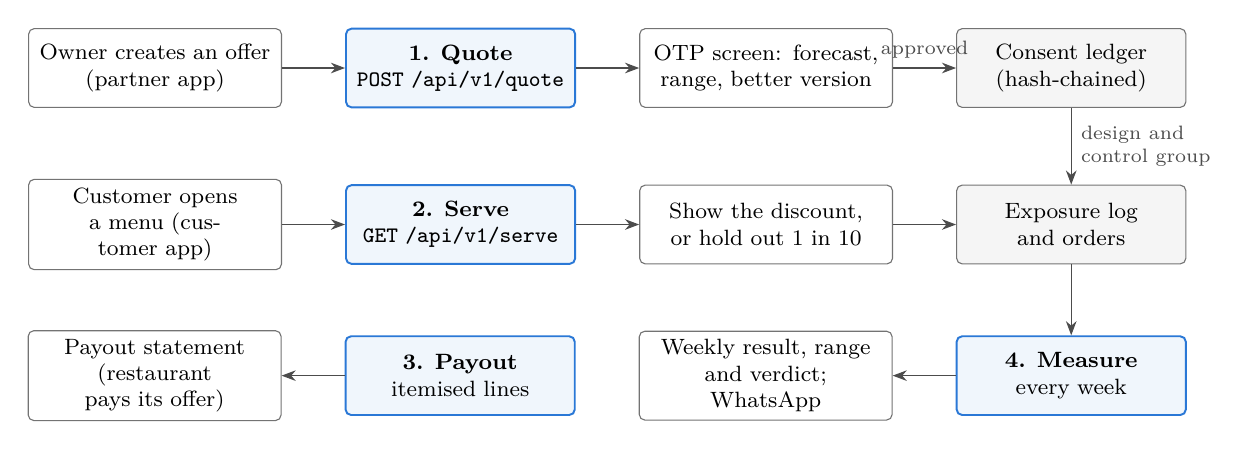
\begin{tikzpicture}[
  box/.style={draw=black!55, rounded corners=2pt, align=center, font=\footnotesize, inner sep=3pt, minimum height=10mm, text width=30mm, fill=white},
  hook/.style={draw=tlblue, line width=0.7pt, fill=tlblue!7, rounded corners=2pt, align=center, font=\footnotesize, inner sep=3pt, minimum height=10mm, text width=27mm},
  store/.style={draw=black!55, fill=black!4, rounded corners=2pt, align=center, font=\footnotesize, inner sep=3pt, minimum height=10mm, text width=27mm},
  arr/.style={-{Stealth[length=1.8mm]}, black!70},
  lane/.style={font=\footnotesize\itshape, text=black!55, anchor=east},
  node distance=5mm and 8mm]
\node[box] (create) {Owner creates an offer\\(partner app)};
\node[hook, right=of create] (quote) {\textbf{1. Quote}\\\texttt{POST /api/v1/quote}};
\node[box, right=of quote] (otp) {OTP screen: forecast,\\range, better version};
\node[store, right=of otp] (ledger) {Consent ledger\\(hash-chained)};
\node[box, below=9mm of create] (menu) {Customer opens\\a menu (customer app)};
\node[hook, right=of menu] (serve) {\textbf{2. Serve}\\\texttt{GET /api/v1/serve}};
\node[box, right=of serve] (decide) {Show the discount,\\or hold out 1 in 10};
\node[store, right=of decide] (log) {Exposure log\\and orders};
\node[hook, below=9mm of log] (measure) {\textbf{4. Measure}\\every week};
\node[box, left=of measure] (result) {Weekly result, range\\and verdict; WhatsApp};
\node[hook, left=of result] (payout) {\textbf{3. Payout}\\itemised lines};
\node[box, left=of payout] (statement) {Payout statement\\(restaurant pays its offer)};
\draw[arr] (create) -- (quote);
\draw[arr] (quote) -- (otp);
\draw[arr] (otp) -- node[above, font=\scriptsize] {approved} (ledger);
\draw[arr] (menu) -- (serve);
\draw[arr] (serve) -- (decide);
\draw[arr] (decide) -- (log);
\draw[arr] (ledger.south) -- node[right, font=\scriptsize, align=left] {design and\\control group} (log.north);
\draw[arr] (log) -- (measure);
\draw[arr] (measure) -- (result);
\draw[arr] (payout) -- (statement);
\end{tikzpicture}
\caption{The four calls TrueLift adds to Zomato's existing offer flow. Blue boxes are TrueLift's
service; the rest exists today. No new screen is needed: the forecast sits on the OTP screen, the
result arrives on WhatsApp, and nothing changes in how customers order. An approval lasts four weeks;
renewing it needs a new OTP and shows what was measured.}
\label{fig:arch}
\end{figure*}

\begin{figure*}[t]
\centering
\includegraphics[width=0.215\textwidth]{img/owner_forecast.png}\hfill
\includegraphics[width=0.215\textwidth]{img/owner_better.png}\hfill
\includegraphics[width=0.215\textwidth]{img/owner_otp.png}\hfill
\includegraphics[width=0.215\textwidth]{img/owner_result.png}
\caption{The owner's flow in the prototype, left to right: (a) the forecast of the owner's usual ₹60-off
offer, with its range and the share of orders that would come anyway; (b) TrueLift's better version
of the same discount; (c) the OTP approval, which records exactly what was shown; (d) the result after
four weeks beside what today's offer report would show. The restaurant is a real 2019 listing; its
customers and money are simulated.}
\label{fig:owner}
\end{figure*}

\emph{1) Quote, before approval.} For the owner's offer, flat (``₹60 off'') or a percentage with a cap,
the service forecasts the extra orders and profit with an 80\% range and compares about 34 versions of
the same discount. It suggests the best one, or says that no version is likely to pay.

\emph{2) Serve, while the offer runs.} When a customer opens the menu, a table lookup built at approval
decides whether the customer sees the discount. A hash of (customer, offer) holds out a random 10\% of
eligible customers for the offer's whole life. Held-out customers see normal menu prices, never higher
ones.

\emph{3) Payout.} The restaurant pays for its own offer, with discount, Brand Pack rewards, commission
and GST itemised. Zomato co-funds only where its own measurement shows a gain.

\emph{4) Measure, every week.} The shown and held-out customers are compared, combined with the model,
and the owner receives the extra profit with a range and a verdict: keep, too early, probably losing,
or pause. The approval lasts four weeks; renewal needs a new OTP and shows what was measured, as the
restaurant associations asked \cite{angelone}.

\emph{Privacy and fairness.} The model reads only order and visit history on Zomato, the restaurant's
public listing, the time of the visit and the offer. It never reads location below the city, device,
payment method or anything that stands in for income, following consumer-authority notices to
ride-hailing apps over phone-based price differences \cite{ccpa}. A test fails if the model reads any
other input.

\section{Method}
\label{sec:method}

\subsection{Uplift model}
For one customer opening one restaurant's menu, two gradient-boosted classifiers \cite{sklearn}
estimate the chance of ordering without an offer, $p_0$, learned from visits that saw none, and with a
given offer, $p_1$, learned from visits that saw one, with the offer's size and minimum order as inputs
(a T-learner \cite{kunzel}). Known directions are enforced as monotone constraints: a bigger discount or
reward never lowers $p_1$, a higher minimum order never raises it. Forecast gains are scaled by
calibration factors learned, cross-fitted, from the shadow phase's random holdouts.

\subsection{Forecast}
Over the visits of the last two weeks that would see the offer,
\begin{align}
\text{extra orders} &= \textstyle\sum (p_1-p_0),\\
\text{extra profit} &= \textstyle\sum (p_1\,\pi_1-p_0\,\pi_0),\\
\text{orders using it} &= \textstyle\sum p_1\,u,
\end{align}
where $\pi_1$ and $\pi_0$ are the restaurant's profit per order with and without the offer and $u$ is
the share of customers who use it. With a minimum order $M$, a customer whose usual order $b$ is below
$M$ uses a ₹$D$ offer only if $D>(1-v)(M-b)$, where $v$ is how much of a top-up they value; TrueLift
learns $v$ from past minimum-order offers and recovers the simulator's hidden value (\V{devlog_topup}).
The range is the model's error measured on past offers that had a random holdout.

\subsection{A better version of the same discount}
The versions compared all keep the owner's discount size and format: with or without a minimum order,
four audiences (everyone, new to the restaurant, stopped ordering for four weeks or more, chosen by
TrueLift), all day or 3--6~pm, with or without a Brand Pack reward, plus ``no offer'' and ``Brand Pack
only''. A version is suggested only if it has at least a 60\% chance of making the owner money.

TrueLift does not choose the discount size. Letting the model also choose it raises restaurants'
profit from their own offers from \V{depth_owner_own} to \V{depth_model_own} a week, but across the
market by only \V{depth_market_gain}, and the offers that lose money rise from \V{depth_lose_before}
to \V{depth_lose_after}: deeper discounts mostly win orders from other restaurants, and past offers vary
the size only between restaurant-weeks, never between customers. A size change should come from a
test that gives customers one size or another at random.

Picking the best of about 34 forecasts favours the ones that came out high. The suggested version
truly beats the owner's at \V{selection_truly_better} of restaurants, but its stated advantage is about
\V{selection_inflation} times its true advantage (\V{selection_stated} against \V{selection_true} a week
across the market). The page therefore shows every suggestion's range and says that the gain may be
smaller in practice.

\subsection{Who sees the discount}
A customer sees the discount only if it is expected to raise the restaurant's profit from that visit.
Regulars who would order anyway therefore rarely get it; a Brand Pack reward, measured with its own
control group, keeps them.

\subsection{Weekly measurement for a small restaurant}
A 10\% holdout alone is too small. With 1,000 eligible visits a week, 7\% ordering without the offer
and 10\% with it, the 95\% range of the measured lift is $\pm$\V{precision_1w} points after one week,
$\pm$\V{precision_4w} after four weeks, $\pm$\V{precision_20pct_4w} with a 20\% holdout over four weeks,
and $\pm$\V{precision_pooled} for 50 similar restaurants pooled over one week. TrueLift therefore
combines the restaurant's own estimate $\hat\Delta_{\text{own}}$ with the model's $\hat\Delta_{\text{model}}$,
each weighted by its precision:
\begin{equation}
\hat\Delta = w\,\hat\Delta_{\text{own}}+(1-w)\,\hat\Delta_{\text{model}},\qquad
w=\frac{\sigma^2_{\text{model}}}{\sigma^2_{\text{model}}+\mathrm{se}^2_{\text{own}}}.
\end{equation}
In week one the model dominates; as the restaurant's own evidence grows, $w$ rises. Both noise sizes are
re-estimated every week across all running offers without the truth: two random halves of each offer's
customers give the noise of its own estimate, and the spread of own estimates around the model's gives
the model's error. Before shown and held-out customers are compared, each visit's predicted no-offer
outcome is subtracted (regression adjustment, as in CUPED \cite{cuped}), which keeps the comparison
unbiased and cuts the noise by \V{noise_cut}.

\subsection{Verdicts and pauses}
No offer is paused on the model's word. A pause needs the offer's own control group to show a loss
beyond a one-sided boundary from a normal-mixture confidence sequence \cite{howard}, which stays valid
however often the owner looks. Renewal after four weeks needs a new OTP.

\section{Experimental Setup}
\label{sec:setup}

No public dataset has restaurant offers with rupee outcomes and a control group, so we built a market
where the truth is known. It has 300 real Bengaluru delivery restaurants (name, locality, cuisine, cost
for two, rating; Kaggle 2019 \cite{kaggle}) in six localities, and 30,000 synthetic customers of four
hidden types (loyal, casual, deal-seeker, infrequent). Each time a customer wants food they look at
eight menus and choose one restaurant, Swiggy, or nothing, by a multinomial logit \cite{mcfadden}.
Because the simulator knows every customer's chance of ordering with and without each discount, it
knows the true effect of every offer. The models never see the hidden types, only order history, as
Zomato would.

The models learn from twelve weeks: eight weeks of today's market, in which 40\% of restaurants run
blanket offers, and a four-week shadow phase in which the offers owners run vary at random over the
create screen's options, with a 10\% holdout; about one million menu visits. Every policy then runs
for four weeks on the same customer visits. We compare TrueLift with \emph{blanket} offers (today: the
same discount for everyone) and a strong \emph{rule} (new customers only). An offer \emph{pays} if its
own effect on its restaurant's profit is positive with the other restaurants' offers unchanged.
TrueLift's figures include the cost of its own control group; the baselines measure nothing.

\section{Results}
\label{sec:results}

\subsection{The market}
Table~\ref{tab:results} and Fig.~\ref{fig:market} give the results per week across all 300 restaurants.
\V{tl_pay} of TrueLift's \V{tl_offers} offers pay for themselves, against \V{bl_pay} of 300 blanket
offers, and TrueLift advises no discount at the other \V{tl_no_offer} restaurants. Of the orders using
a blanket offer, \V{bl_anyway} would have come anyway; with TrueLift, \V{tl_anyway}. Across
\V{method_seeds_count} market seeds TrueLift beats blanket offers on offers that pay, own-offer profit,
market-wide restaurant profit and Zomato's commission in every seed, with about ₹\V{seeds_less_discount}
lakh a week less discount. Zomato gains because offers that pay keep being approved: under the OTP rule,
\V{bl_lose} of the 300 blanket offers lose their restaurant money. Of the extra orders TrueLift creates,
\V{tl_platform_share} are extra for Zomato as a whole (\V{bl_platform_share} for blanket offers). Holding
out one customer in ten costs \V{control_group_profit} of restaurant profit a week across the market
(\V{control_group_orders} orders): the price of knowing what each offer adds.

\begin{table}[t]
\caption{Results per week, 300 simulated restaurants (money in ₹ lakh)}
\label{tab:results}
\centering\footnotesize
\setlength{\tabcolsep}{3pt}
\begin{tabular}{@{}L{30mm}R{15mm}R{15mm}R{15mm}@{}}
\toprule
& Blanket (today) & Rule: new customers & TrueLift \\
\midrule
\TabResults
\bottomrule
\end{tabular}
\end{table}

\begin{figure}[t]
\centering
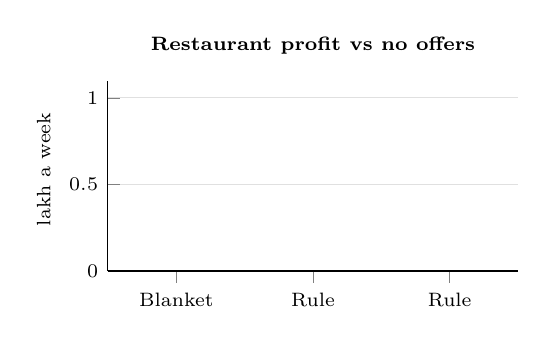
\begin{tikzpicture}
\begin{axis}[ybar, width=0.56\columnwidth, height=40mm, bar width=7mm, ymin=0,
  symbolic x coords={Blanket,Rule,TrueLift}, xtick={Blanket,Rule,TrueLift}, enlarge x limits=0.25,
  nodes near coords, nodes near coords style={font=\scriptsize, /pgf/number format/fixed, /pgf/number format/fixed zerofill, /pgf/number format/precision=2},
  ylabel={₹ lakh a week}, ylabel style={font=\scriptsize}, tick label style={font=\scriptsize},
  title={Restaurant profit vs no offers}, title style={font=\scriptsize\bfseries},
  axis lines*=left, ymajorgrids, grid style={black!12}]
\addplot[fill=tlgrey, draw=none, bar shift=0pt] coordinates {\CoordMarketBase};
\addplot[fill=tlblue, draw=none, bar shift=0pt] coordinates {\CoordMarketTL};
\end{axis}
\end{tikzpicture}\hspace{-2mm}%
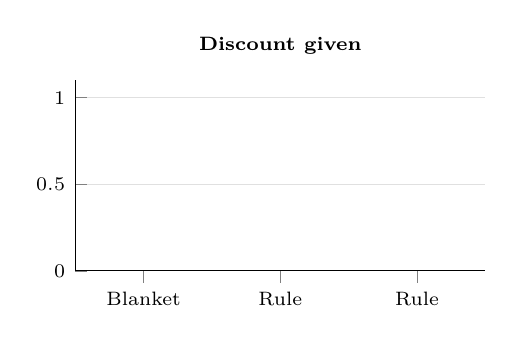
\begin{tikzpicture}
\begin{axis}[ybar, width=0.56\columnwidth, height=40mm, bar width=7mm, ymin=0,
  symbolic x coords={Blanket,Rule,TrueLift}, xtick={Blanket,Rule,TrueLift}, enlarge x limits=0.25,
  nodes near coords, nodes near coords style={font=\scriptsize, /pgf/number format/fixed, /pgf/number format/fixed zerofill, /pgf/number format/precision=2},
  tick label style={font=\scriptsize},
  title={Discount given}, title style={font=\scriptsize\bfseries},
  axis lines*=left, ymajorgrids, grid style={black!12}]
\addplot[fill=tlgrey, draw=none, bar shift=0pt] coordinates {\CoordDiscountBase};
\addplot[fill=tlblue, draw=none, bar shift=0pt] coordinates {\CoordDiscountTL};
\end{axis}
\end{tikzpicture}
\caption{TrueLift raises restaurants' profit over no offers while giving far less discount than
blanket offers (₹ lakh a week, 300 restaurants). Values from Table~\ref{tab:results}.}
\label{fig:market}
\end{figure}

\subsection{Is the forecast right?}
In today's market, where one restaurant switches while the others keep their offers (the condition a
quote describes), TrueLift's forecasts add up to \V{forecast_ratio} of the true effect of the versions
it chose; \V{forecast_coverage} of the true effects fall inside the 80\% ranges, and the sign is right
for \V{forecast_sign} of offers. The forecast is cautious and its ranges are wide.

\subsection{Are the weekly numbers right?}
Table~\ref{tab:measure} and Fig.~\ref{fig:error} compare each offer's running estimate of extra profit
with the truth. The combined estimate's error is below both of its parts from week one, and its 80\%
range holds the truth \V{devlog_cov_1}, \V{devlog_cov_2} and \V{devlog_cov_4} of the time after one, two
and four weeks. Placebo offers, which change nothing, were paused in \V{aa_4_looks} of cases over a
four-week approval (\V{aa_4_looks_before} under the earlier rule ``pause when the range is below zero'')
and in \V{aa_12_looks} over twelve weekly looks (\V{aa_12_looks_before} before). Across ten random holdout
draws the four-week estimate over-states the truth by \V{draws_bias} an offer on average (standard error
\V{draws_bias_se}), a bias inherited from the model while an offer's own control group is small.

\begin{table}[t]
\caption{Weekly measurement against the truth (TrueLift's offers)}
\label{tab:measure}
\centering\scriptsize
\setlength{\tabcolsep}{2.5pt}
\begin{tabular}{@{}L{10mm}R{11mm}R{12mm}R{10mm}R{12mm}R{14mm}@{}}
\toprule
After & Truth in 80\% range & Error: control only & Model only & TrueLift combined & ``Keep'' truly positive \\
\midrule
\TabMeasurement
\bottomrule
\end{tabular}
\end{table}

\begin{figure}[t]
\centering
\begin{tikzpicture}
\begin{axis}[width=0.95\columnwidth, height=44mm, xmin=0.7, xmax=4.3, ymin=0, xtick={1,2,4},
  xlabel={Weeks since approval}, ylabel={Average error (₹)}, label style={font=\scriptsize},
  tick label style={font=\scriptsize}, axis lines*=left, ymajorgrids, grid style={black!12},
  legend style={font=\scriptsize, draw=none, at={(0.5,1.03)}, anchor=south, legend columns=3,
    /tikz/every even column/.append style={column sep=2mm}},
  yticklabel style={/pgf/number format/fixed, /pgf/number format/1000 sep={,}}]
\addplot[tldark, densely dashed, mark=o, mark size=1.6pt, line width=0.8pt] coordinates {\CoordErrown};
\addplot[tlgrey, mark=square*, mark size=1.5pt, line width=0.8pt] coordinates {\CoordErrmodel};
\addplot[tlblue, mark=*, mark size=1.8pt, line width=1.2pt] coordinates {\CoordErrcomb};
\legend{Control group only, Model only, TrueLift combined}
\end{axis}
\end{tikzpicture}
\caption{Average absolute error of the running estimate of an offer's extra profit. Combining the
restaurant's own control group with the model beats both parts in every week.}
\label{fig:error}
\end{figure}

\subsection{Does the model find whom a discount moves?}
On the evaluation weeks the predicted uplift per visit correlates \V{uplift_corr} with the true uplift
(Qini \V{uplift_qini}, where 0 is a random ranking). Over five simulated markets the T-learner earns
the most profit from its top 30\% of any learner (\V{bench_t_profit} of the best possible), against
\V{bench_response_profit} for ranking by who is likely to order anyway. With one fixed discount
everywhere, its targeting captures \V{oracle_share} of what an oracle that knows every visit's true
response could add over blanket offers.

\subsection{Robustness}
Table~\ref{tab:scen} varies price sensitivity by $\pm$30\% and charges commission before the discount.
TrueLift has the most paying offers in every case but the last, where the rule has slightly more, and
the highest market-wide restaurant profit in every case. A sweep of eight assumptions, each low and high,
is in the repository with where each claim stops holding.

\begin{table*}[t]
\caption{Scenarios, per week: blanket / rule / TrueLift}
\label{tab:scen}
\centering\scriptsize
\setlength{\tabcolsep}{3pt}
\begin{tabular}{@{}L{40mm}L{22mm}L{50mm}L{52mm}@{}}
\toprule
Scenario & Offers that pay & Restaurants' profit from their own offers & Restaurant profit vs no offers (market) \\
\midrule
\TabScenarios
\bottomrule
\end{tabular}
\end{table*}

\subsection{Real randomised data}
The same method, refitted on each dataset, ranked customers it had never seen in two public randomised
experiments: Criteo's advertising tests (\V{criteo_rows} million users, a random 15\% held out of ads)
\cite{criteo} and Hillstrom's retail e-mail test (\V{hillstrom_rows} customers) \cite{hillstrom}. Table~\ref{tab:real}
reports the share of each campaign's total extra outcome found in the top 30\% of each ranking, with
90\% intervals from 200 resamples. On Criteo's visits every ranking, including the shortcut of ranking
people by how likely they are to act at all, finds about the same share; on Criteo's rare purchases the
shortcut does best. On Hillstrom's women's e-mail the uplift models find more than the shortcut in all
five random splits. On dollars spent no ranking is reliably better than random with about
\V{hillstrom_test_rows} test customers per e-mail, which is why TrueLift models the chance of an order
and computes the money from each order's economics. Neither dataset is about food discounts: they test
the method, not Zomato's numbers.

\begin{table*}[t]
\caption{Real randomised data: share of all extra response found in the top 30\% of each ranking (90\% interval)}
\label{tab:real}
\centering\scriptsize
\setlength{\tabcolsep}{4pt}
\begin{tabular}{@{}lrrrrr@{}}
\toprule
Dataset and outcome & Random & Likely to act anyway & S-learner & T-learner (TrueLift) & X-learner \\
\midrule
\TabRealData
\bottomrule
\end{tabular}
\end{table*}

\subsection{A caution on platform co-funding}
Paying half the discount for customers new to Zomato, with the same customers shown the offer, costs
Zomato \V{cofund_transfer} a week and creates no extra order: the customer sees the same offer whoever
pays for it. Zomato should co-fund only where a platform-level holdout shows new customers it would not
otherwise get, and pay per measured extra customer, not per redemption.

\section{Prototype}
\label{sec:prototype}

The service (Python, FastAPI) exposes the four calls under \texttt{/api/v1} with a typed contract,
problem-detail errors, per-visitor sessions, OTP expiry and attempt limits, a hash-chained consent
ledger, an exposure log that the measurement reads, and health, readiness and metrics endpoints. It runs
locally or in Docker. The partner-app screens follow Zomato's style: create an offer with a live
forecast and a better version, approve it with an OTP, and read weekly results, the evidence behind them,
the WhatsApp text and the itemised payout. An ``Inside Zomato'' panel shows the restaurant's visitors
(synthetic people), whether each sees the discount, and the simulator's truth beside TrueLift's estimate.
A ten-step guided demo tells the story with captions.

The public demo is a static copy of the service's own answers for 32 restaurants and every offer the
create screen allows; an offline copy runs without internet. Table~\ref{tab:latency} gives speeds measured
over HTTP on a laptop with \V{lat_cpus} logical CPUs. The quote is shown to an owner, not on a customer's
path; inside Zomato it would be computed in batch.

\begin{table}[t]
\caption{Speed over HTTP on a laptop (milliseconds)}
\label{tab:latency}
\centering\footnotesize
\begin{tabular}{@{}lrrr@{}}
\toprule
& Median & 95th pct. & 99th pct. \\
\midrule
Serve one customer & \V{lat_serve_p50} & \V{lat_serve_p95} & \V{lat_serve_p99} \\
Serve, inside the service & \V{lat_inside_p50} & \V{lat_inside_p95} & \V{lat_inside_p99} \\
Serve, eight callers at once & \V{lat_8_p50} & \V{lat_8_p95} & \V{lat_8_p99} \\
Quote: forecast and 34 versions & \V{lat_quote_p50} & \V{lat_quote_p95} & \V{lat_quote_p99} \\
\bottomrule
\end{tabular}
\end{table}

\emph{Engineering checks.} Tests cover each area, golden numbers, contract fuzzing and browser tests on
Linux and Windows. Every number in the documents is checked against the reports by a ledger of
\V{claims_count} claims, and this report's numbers are filled from the same ledger, so no document can
disagree with the results. An audit of our own work found 50 issues; each is fixed and guarded by a test.

\section{From Prototype to Pilot}
Inside Zomato the first step changes nothing for owners: a shadow holdout of 2\% of eligible customers
on offers owners already run, in one city, measured with the same estimator. Next, a randomised pilot of
the forecast and weekly result needs \V{pilot_per_arm} restaurants in each half (\V{pilot_total} in all).
Owners in that half may then let TrueLift choose who sees the offer, and the system scales city by city
with the same guardrails: sample-ratio checks, placebo offers and the renewal rate. Each phase starts only
when the one before has passed its checks.

\section{Limitations and Ethics}
All outcomes are simulated; customer types, price sensitivity and the Swiggy option are our assumptions,
varied in the sensitivity sweep, and real numbers need Zomato's data. The real-data checks are
advertising and e-mail, not food discounts. Not modelled: Swiggy reacting, kitchen capacity, delivery
fees, platform coupons stacking with restaurant offers, and habits that change over months. The
suggested version's stated advantage runs well above its true advantage, and the weekly estimate leans on
the model while a restaurant's own control group is small.

Restaurant names and listing details are real public 2019 listings; every customer, order and profit is
simulated, and every screen says so. No real customer data is used. Regulars are offered fewer discounts
because they order anyway: loyal customers move slightly more to Swiggy than under blanket offers
(\V{tl_swiggy_loyal} of their visits against \V{bl_swiggy_loyal}) and less than with no offers at all
(\V{no_offer_swiggy_loyal}); a Brand Pack reward measured on its own closes the gap at almost no cost.
We have begun interviews with restaurant owners; the first took place on 17 November 2026, and we
report no finding until its note is written up.

\section{Conclusion}
Under consent-based discounting, an owner approves an offer only if they believe it pays. TrueLift makes
that belief checkable: a forecast with an honest range before the OTP, a discount shown to the customers
it moves, a random control group that keeps the result honest, and a weekly measurement that holds the
truth inside its range about as often as it promises. In a market with known truth, the offers that lose
money fall from \V{bl_lose} of 300 under blanket offers to \V{tl_lose} with TrueLift, with far less
discount, and Zomato's commission rises because good offers keep being approved. The next step is a
shadow holdout on real offers.

\begin{thebibliography}{99}
\bibitem{eternal} Eternal Ltd., ``Shareholders' letter: Q2 FY27 results,'' Oct. 2026. [Online]. Available: \url{https://b.zmtcdn.com/investor-relations/Eternal_Limited_Shareholders_Letter_Q2FY27_Results.pdf}
\bibitem{angelone} Angel One, ``Swiggy, Zomato agree to consent-based discounts; Bengaluru hotel bodies defer boycott to September 1,'' Aug. 8, 2026.
\bibitem{theweek} The Week, ``Won't take orders anymore: why Bengaluru restaurants are threatening to boycott Zomato, Swiggy,'' Jul. 30, 2026.
\bibitem{kunzel} S. R. K\"unzel, J. S. Sekhon, P. J. Bickel, and B. Yu, ``Metalearners for estimating heterogeneous treatment effects using machine learning,'' \emph{Proc. Natl. Acad. Sci.}, vol. 116, no. 10, pp. 4156--4165, 2019.
\bibitem{radcliffe} N. J. Radcliffe, ``Using control groups to target on predicted lift: Building and assessing uplift models,'' \emph{Direct Marketing Analytics Journal}, vol. 1, pp. 14--21, 2007.
\bibitem{criteo} E. Diemert, A. Betlei, C. Renaudin, M.-R. Amini, T. Gregoir, and T. Rahier, ``A large scale benchmark for individual treatment effect prediction and uplift modeling,'' arXiv:2111.10106, 2021.
\bibitem{hillstrom} K. Hillstrom, ``The MineThatData e-mail analytics and data mining challenge,'' MineThatData, 2008.
\bibitem{cuped} A. Deng, Y. Xu, R. Kohavi, and T. Walker, ``Improving the sensitivity of online controlled experiments by utilizing pre-experiment data,'' in \emph{Proc. 6th ACM Int. Conf. Web Search and Data Mining (WSDM)}, 2013, pp. 123--132.
\bibitem{howard} S. R. Howard, A. Ramdas, J. McAuliffe, and J. Sekhon, ``Time-uniform, nonparametric, nonasymptotic confidence sequences,'' \emph{Ann. Statist.}, vol. 49, no. 2, pp. 1055--1080, 2021.
\bibitem{ghostads} G. A. Johnson, R. A. Lewis, and E. I. Nubbemeyer, ``Ghost ads: Improving the economics of measuring online ad effectiveness,'' \emph{J. Marketing Research}, vol. 54, no. 6, pp. 867--884, 2017.
\bibitem{doordash} DoorDash Ads, ``Measuring restaurant ads incrementality with ghost ads.'' [Online]. Available: \url{https://advertising.doordash.com/en-ca/resources/measuring-incrementality-with-ghost-ads-at-doordash}
\bibitem{swiggy} Swiggy, ``Discount Self Serve,'' Swiggy Blog, Apr. 2024. [Online]. Available: \url{https://blog.swiggy.com/?p=18470}
\bibitem{brandpacks} Business Standard, ``Zomato rolls out Brand Packs to reward repeat orders from restaurants,'' Jul. 2024.
\bibitem{ccpa} Business Standard, ``CCPA issues notices to Ola, Uber over differential pricing practice,'' Jan. 2025.
\bibitem{sklearn} F. Pedregosa \emph{et al.}, ``Scikit-learn: Machine learning in Python,'' \emph{J. Mach. Learn. Res.}, vol. 12, pp. 2825--2830, 2011.
\bibitem{mcfadden} D. McFadden, ``Conditional logit analysis of qualitative choice behavior,'' in \emph{Frontiers in Econometrics}, P. Zarembka, Ed. New York: Academic Press, 1974, pp. 105--142.
\bibitem{kaggle} H. Poddar, ``Zomato Bangalore Restaurants,'' Kaggle dataset, 2019. [Online]. Available: \url{https://www.kaggle.com/datasets/himanshupoddar/zomato-bangalore-restaurants}
\end{thebibliography}

\end{document}
